\chapter{Sequences and Strings}
\label{chap:chapter4}
\minitoc

\setcounter{lstlisting}{5}

In this chapter you will begin to write Perl programs that manipulate biological sequence data, that is, DNA and proteins. Once you have the sequences in the computer, you'll start writing programs that do the following with the sequence data:

\begin{itemize}
  \item Transcribe DNA to RNA
  \item Concatenate sequences
  \item Make the reverse complement of sequences
  \item Read sequence data from files
\end{itemize}

You'll also write programs that give information about your sequences. How GC-rich is your DNA? How hydrophobic is your protein? You'll see programming techniques you can use to answer these and similar questions.

The Perl skills you will learn in this chapter involve the basics of the language. Here are some of those basics:

\begin{itemize}
  \item Scalar variables
  \item Array variables
  \item String operations such as substitution and translation
  \item Reading data from files
\end{itemize}

\section{Representing Sequence Data}
The majority of this book deals with manipulating symbols that represent the biological sequences of DNA and proteins. The symbols used in bioinformatics to represent these sequences are the same symbols biologists have been using in the literature for this same purpose.

As stated earlier, DNA is composed of four building blocks: the nucleic acids, also called nucleotides or bases. Proteins are composed of 20 building blocks, the amino acids, also called residues. Fragments of proteins are called peptides. Both DNA and proteins are essentially polymers, made from their building blocks attached end to end. So it's possible to summarize the structure of a DNA molecule or protein by simply giving the sequence of bases or amino acids.

These are brief definitions; I'm assuming you are either already
familiar with them or are willing to consult an introductory textbook on
molecular biology for more specific details. \autoref{tab:table4.1} shows bases; add a sugar and you get the nucleotides adenosine, guanosine, cytidine, thymidine, and uridine. You can further add a phosphate and get the nucleotides adenylic acid, guanylic acid, cytidylic acid, thymidylic acid, and uridylic acid. A nucleic acid is a chemically linked sequence of nucleotides. A peptide is a small number of joined amino acids; a longer chain is a polypeptide. A protein is a biologically functional unit made of one or more polypeptides. A residue is an amino acid in a polypeptide chain.

For expediency, the names of the nucleic acids and the amino acids are
often represented as one- or three-letter codes, as shown in
\autoref{tab:table4.1} and \autoref{tab:table4.2}. (This book mostly uses the one-letter codes for amino acids.) 

\begin{table}[!htbp]
  \begin{center}
  \caption{Standard IUB/IUPAC nucleic acid codes}
  \label{tab:table4.1}
  %\begin{tabu}{X[1,c]X[2,l]}
  \begin{tabu} to 0.5\linewidth {X[1,c]X[2,c]}
  \toprule
  Code & Nucleic Acid(s)\\
  \midrule
  A & Adenine\\
  C & Cytosine\\
  G & Guanine\\
  T & Thymine\\
  U & Uracil\\
  M & A or C (amino)\\
  R & A or G (purine)\\
  W & A or T (weak)\\
  S & C or G (strong)\\
  Y & C or T (pyrimidine)\\
  K & G or T (keto)\\
  V & A or C or G\\
  H & A or C or T\\
  D & A or G or T\\
  B & C or G or T\\
  N & A or G or C or T (any)\\
  \bottomrule
  \end{tabu}
  \end{center}
\end{table}

The nucleic acid codes in \autoref{tab:table4.1} include letters for the four basic nucleic acids; they also define single letters for all possible groups of two, three, or four nucleic acids. In most cases in this book, I use only A, C, G, T, U, and N. The letters A, C, G, and T represent the nucleic acids for DNA. U replaces T when DNA is transcribed into ribonucleic acid (RNA). N is the common representation for "unknown," as when a sequencer can't determine a base with certainty. Later on, in \autoref{chap:chapter9}, we'll need the other codes, for groups of nucleic acids, when programming restriction maps. Note that the lowercase versions of these single-letter codes is also used on occasion, frequently for DNA, rarely for protein. 

\begin{table}[!htbp]
  \begin{center}
  \caption{Standard IUB/IUPAC amino acid codes}
  \label{tab:table4.2}
  %\begin{tabu}{X[1,c]X[2,l]}
  \begin{tabu} to 0.8\linewidth {X[1,c]X[2,c]X[1,c]}
  \toprule
  One-letter code & Amino acid & Three-letter code\\
  \midrule
  A & Alanine & Ala\\
  B & Aspartic acid or Asparagine & Asx\\
  C &  Cysteine & Cys\\
  D & Aspartic acid &  Asp\\
  E & Glutamic acid & Glu\\
  F & Phenylalanine & Phe\\
  G & Glycine & Gly\\
  H & Histidine & His\\
  I & Isoleucine & Ile\\
  K & Lysine & Lys\\
  L & Leucine & Leu\\
  M & Methionine & Met\\
  N & Asparagine & Asn\\
  P & Proline & Pro\\
  Q & Glutamine & Gln\\
  R & Arginine & Arg\\
  S & Serine & Ser\\
  T & Threonine & Thr\\
  V & Valine & Val\\
  W & Tryptophan & Trp\\
  X & Unknown & Xxx\\
  Y & Tyrosine & Tyr\\
  Z & Glutamic acid or Glutamine & Glx\\
  \bottomrule
  \end{tabu}
  \end{center}
\end{table}

The computer-science terminology is a little different from the biology terminology for the codes in \autoref{tab:table4.1} and \autoref{tab:table4.2}. In computer-science parlance, these tables define two alphabets, finite sets of symbols that can make strings. A sequence of symbols is called a string. For instance, this sentence is a string. A language is a (finite or infinite) set of strings. In this book, the languages are mainly DNA and protein sequence data. You often hear bioinformaticians referring to an actual sequence of DNA or protein as a "string," as opposed to its representation as sequence data. This is an example of the terminologies of the two disciplines crossing over into one another.

As you've seen in the tables, we'll be representing data as simple letters, just as written on a page. But computers actually use additional codes to represent simple letters. You won't have to worry much about this; just remember that when using your text editor to save as ASCII, or plain text.

ASCII is a way for computers to store textual (and control) data in their memory. Then when a program such as a text editor reads the data, and it knows it's reading ASCII, it can actually draw the letters on the screen in a recognizable fashion because it's programmed to know that particular code. So the bottom line is: ASCII is a code to represent text on a computer.\footnote{A new character encoding called Unicode, which can handle all the symbols in all the world's languages, is becoming widely accepted and is supported by Perl as well.}

\section{A Program to Store a DNA Sequence}
Let's write a small program that stores some DNA in a variable and prints it to the screen. The DNA is written in the usual fashion, as a string made of the letters A, C, G, and T, and we'll call the variable \verb|$DNA|. In other words, \verb|$DNA| is the name of the DNA sequence data used in the program. Note that in Perl, a variable is really the name for some data you wish to use. The name gives you full access to the data. \autoref{exam:example4.1} shows the entire program.

\textbf{Example 4-1. Putting DNA into the computer}
\lstinputlisting[label=exam:example4.1]{./scripts/example4-1.pl}

Using what you've already learned about text editors and running Perl programs in \autoref{chap:chapter2}, enter the code (or copy it from the book's web site) and save it to a file. Remember to save the program as ASCII or text-only format, or Perl may have trouble reading the resulting file.

The second step is to run the program. The details of how to run a program depend on the type of computer you have (see \autoref{chap:chapter2}). Let's say the program is on your computer in a file called \textit{example4-1}. As you recall from \autoref{chap:chapter2}, if you are running this program on Unix or Linux, you type the following in a shell window:

\verb|perl example4-1 |

On a Mac, open the file with the MacPerl application and save it as a droplet, then just double-click on the droplet. On Windows, type the following in an MS-DOS command window: 

\verb|perl example4 -1|

If you've successfully run the program, you'll see the output printed on your computer screen. 

\subsection{Control Flow}
\autoref{exam:example4.1} illustrates many of the ideas all our Perl programs will rely on. One of these ideas is \textit{control flow}, or the order in which the statements in the program are executed by the computer.

Every program starts at the first line and executes the statements one after the other until it reaches the end, unless it is explicitly told to do otherwise. \autoref{exam:example4.1} simply proceeds from top to bottom, with no detours.

In later chapters, you'll learn how programs can control the flow of execution. 

\subsection{Comments Revisited}
Now let's take a look at the parts of \autoref{exam:example4.1}. You'll notice lots of blank lines. They're there to make the program easy for a human to read.  Next, notice the comments that begin with the \# sign. Remember from \autoref{chap:chapter3} that when Perl runs, it throws these away along with the blank lines. In fact, to Perl, the following is exactly the same program as \autoref{exam:example4.1}: 

\begin{lstlisting}
#!/usr/bin/perl -w
$DNA = 'ACGGGAGGACGGGAAAATTACTACGGCATTAGC'; print $DNA; exit;
\end{lstlisting}

In \autoref{exam:example4.1}, I've made liberal use of comments. Comments at the beginning of code can make it clear what the program is for, who wrote it, and present other information that can be helpful when someone needs to understand the code. Comments also explain what each section of the code is for and sometimes give explanations on how the code achieves its goals.

It's tempting to belabor the point about the importance of comments.  Suffice it to say that in most university-level, computer-science class assignments, the program without comments typically gets a low or failing grade; also, the programmer on the job who doesn't comment code is liable to have a short and unsuccessful career.

\subsection{Command Interpretation}
Because it starts with a \# sign, the first line of the program looks like a comment, but it doesn't seem like a very informative comment:

\begin{lstlisting}
#!/usr/bin/perl -w
\end{lstlisting}

This is a special line called command interpretation that tells the computer running Unix and Linux that this is a Perl program. It may look slightly different on different computers. On some machines, it's also unnecessary because the computer recognizes Perl from other information.  A Windows machine is usually configured to assume that any program ending in \textit{.pl} is a Perl program. In Unix or Linux, a Windows command window, or a MacOS X shell, you can type \verb|perl my_program|, and your Perl program \verb|my_program| won't need the special line. However, it's commonly used, so we'll have it at start all our programs.

Notice that the first line of code uses a flag \verb|-w|. The "w" stands for warnings, and it causes Perl to print messages in case of an error. Very often the error message suggests the line number where it thinks the error began. Sometimes the line number is wrong, but the error is usually on or just before the line the message suggests. Later in the book, you'll also see the statement \verb|use warnings| as an alternative to \verb|-w|. 

\subsection{Statements}
The next line of \autoref{exam:example4.1} stores the DNA in a variable:

\begin{lstlisting}
$DNA = 'ACGGGAGGACGGGAAAATTACTACGGCATTAGC';
\end{lstlisting}

This is a very common, very important thing to do in a computer language, so let's take a leisurely look at it. You'll see some basic features about Perl and about programming languages in general, so this is a good place to stop skimming and actually read.

This line of code is called a \textit{statement}. In Perl, statements end in a semicolon (;). The use of the semicolon is similar to the use of the period in the English language.

To be more accurate, this line of code is an \textit{assignment} statement. Its purpose in this program is to store some DNA into a variable called \verb|$DNA|. There are several fundamental things happening here as you will see in the next sections. 

\subsubsection{Variables}
First, let's look at the variable \verb|$DNA|. Its name is somewhat arbitrary.  You can pick another name for it, and the program behaves the same way.  For instance, if you replace the two lines:

\begin{lstlisting}
$DNA = 'ACGGGAGGACGGGAAAATTACTACGGCATTAGC';
print $DNA;
\end{lstlisting}

with these:

\begin{lstlisting}
$A_poem_by_Seamus_Heaney = 'ACGGGAGGACGGGAAAATTACTACGGCATTAGC';
print $A_poem_by_Seamus_Heaney;
\end{lstlisting}

the program behaves in exactly the same way, printing out the DNA to the computer screen. The point is that the names of variables in a computer program are your choice. (Within certain restrictions: in Perl, a variable name must be composed from upper- or lowercase letters, digits, and the underscore \_ character. Also the first character must not be a digit.)

This is another important point along the same lines as the remarks I've already made about using blank lines and comments to make your code more easily read by humans. The computer attaches no meaning to the use of the variable name \verb|$DNA| instead of \verb|$A_poem_by_Seamus_Heaney|, but whoever reads the program certainly will. One name makes perfect sense, clearly indicates what the variable is for in the program, and eases the chore of understanding the program. The other name makes it unclear what the program is doing or what the variable is for. Using well-chosen variable names is part of what's called self-documenting code. You'll still need comments, but perhaps not as many, if you pick your variable names well.

You've noticed that the variable name \verb|$DNA| starts with dollar sign. In Perl this kind of variable is called a scalar variable, which is a variable that holds a single item of data. Scalar variables are used for such data as strings or various kinds of numbers (e.g., the string \verb|hello| or numbers such as 25, 6.234, 3.5E10, -0.8373). A scalar variable holds just one item of data at a time. 

\subsubsection{Strings}
In \autoref{exam:example4.1}, the scalar variable \verb|$DNA| is holding some DNA, represented in the usual way by the letters A, C, G, and T. As stated earlier, in computer science a sequence of letters is called a string.  In Perl you designate a string by putting it in quotes. You can use single quotes, as in \autoref{exam:example4.1}, or double quotes. (You'll learn the difference later.) The DNA is thus represented by:

\begin{lstlisting}
'ACGGGAGGACGGGAAAATTACTACGGCATTAGC'
\end{lstlisting}

\subsubsection{Assignment}
In Perl, to set a variable to a certain value, you use the = sign. The = sign is called the \textit{assignment operator}. In \autoref{exam:example4.1}, the value: 

\begin{lstlisting}
'ACGGGAGGACGGGAAAATTACTACGGCATTAGC' 
\end{lstlisting}

is assigned to the variable \verb|$DNA|. After the assignment, you can use the name of the variable to get the value, as in the \verb|print| statement in \autoref{exam:example4.1}.  

The order of the parts is important in an assignment statement. The value assigned to something appears to the right of the assignment operator. The variable that is assigned a value is always to the left of the assignment operator. In programming manuals, you sometimes come across the terms \textit{lvalue} and \textit{rvalue} to refer to the left and right sides of the assignment operator.

This use of the = sign has a long history in programming languages.  However, it can be a source of confusion: for instance, in most mathematics, using = means that the two things on either side of the sign are equal. So it's important to note that in Perl, the = sign doesn't mean equality. It assigns a value to a variable. (Later, we'll see how to represent equality.)

So, to summarize what we've learned so far about this statement:

\begin{lstlisting}
$DNA = 'ACGGGAGGACGGGAAAATTACTACGGCATTAGC';
\end{lstlisting}

It's an assignment statement that sets the value of the scalar variable \verb|$DNA| to a string representing some DNA. 

\subsubsection{Print}
The statement:

\begin{lstlisting}
print $DNA;
\end{lstlisting}

prints \verb|ACGGGAGGACGGGAAAATTACTACGGCATTAGC| out to the computer screen.  Notice that the print statement deals with scalar variables by printing out their values—in this case, the string that the variable \verb|$DNA| contains. You'll see more about printing later. 

\subsubsection{Exit}
Finally, the statement \verb|exit;| tells the computer to exit the program.  Perl doesn't require an \verb|exit| statement at the end of a program; once you get to the end, the program exits automatically. But it doesn't hurt to put one in, and it clearly indicates the program is over. You'll see other programs that exit if something goes wrong before the program normally finishes, so the \verb|exit| statement is definitely useful. 

\section{Concatenating DNA Fragments}
  Now we'll make a simple modification of \autoref{exam:example4.1} to show how to concatenate two DNA fragments. Concatenation is attaching something to the end of something else. A biologist is well aware that joining DNA sequences is a common task in the biology lab, for instance when a clone is inserted into a cell vector or when splicing exons together during the expression of a gene. Many bioinformatics software packages have to deal with such operations; hence its choice as an example.

\autoref{exam:example4.2} demonstrates a few more things to do with strings, variables, and print statements. 

\textbf{Example 4-2. Concatenating DNA}
\lstinputlisting[label=exam:example4.2]{./scripts/example4-2.pl}

As you can see, there are three variables here, \verb|$DNA1|, \verb|$DNA2|, and \verb|$DNA3|.  I've added \verb|print| statements for a running commentary, so that the output of the program that appears on the computer screen makes more sense and isn't simply some DNA fragments one after the other.

Here's what the output of Example 4-2 looks like:

\begin{lstlisting}
Here are the original two DNA fragments:

ACGGGAGGACGGGAAAATTACTACGGCATTAGC
ATAGTGCCGTGAGAGTGATGTAGTA

Here is the concatenation of the first two fragments
(version 1):

ACGGGAGGACGGGAAAATTACTACGGCATTAGCATAGTGCCGTGAGAGTGATGTAGTA

Here is the concatenation of the first two fragments
(version 2):

ACGGGAGGACGGGAAAATTACTACGGCATTAGCATAGTGCCGTGAGAGTGATGTAGTA

Here is the concatenation of the first two fragments
(version 3):

ACGGGAGGACGGGAAAATTACTACGGCATTAGCATAGTGCCGTGAGAGTGATGTAGTA
\end{lstlisting}

\autoref{exam:example4.2} has many similarities to \autoref{exam:example4.1}. Let's look at the differences. To start with, the print statements have some extra, unintuitive parts:

\begin{lstlisting}
print $DNA1, "\n";
print $DNA2, "\n\n";
\end{lstlisting}

The \verb|print| statements have variables containing the DNA, as before, but now they also have a comma and then \verb|"\n"| or \verb|"\n\n"|. These are instructions to print newlines. A \textit{newline} is invisible on the page or screen, but it tells the computer to go on to the beginning of the next line for subsequent printing. One newline, \verb|"\n"|, simply positions you at the beginning of the next line. Two new lines, \verb|"\n\n"|, moves to the next line and then positions you at the beginning of the line after that, leaving a blank line in between.  

Look at the code for \autoref{exam:example4.2} and to make sure you see what these newline directives do to the output. A blank line is a line with nothing printed on it. Depending on your operating system, it may be just a newline character or a combination formfeed and carriage return (in which cases, it may also be called an empty line), or it may include nonprinting whitespace characters such as spaces and tabs. Notice that the newlines are enclosed in double quotes, which means they are parts of strings. (Here's one difference between single and double quotes, as mentioned earlier: \verb|"\n"| prints a newline; \verb|'\n'| prints \verb|\n| as written.)

Notice the comma in the print statement. A comma separates items in a list. The print statement prints all the items that are listed. Simple as that.

Now let's look at the statement that concatenates the two DNA fragments \verb|$DNA1| and \verb|$DNA2| into the variable \verb|$DNA3|:

\begin{lstlisting}
$DNA3 = "$DNA1$DNA2"; 
\end{lstlisting}

The assignment to \verb|$DNA3| is just a typical assignment as you saw in \autoref{exam:example4.1}, a variable name followed by the = sign, followed by a value to be assigned.

The value to the right of the assignment statement is a string enclosed in double quotes. The double quotes allow the variables in the string to be replaced with their values. This is called string interpolation.\footnote{There are occasions when you might add curly braces during string interpolation. The extra curly braces make sure the variable names aren't confused with anything else in the double-quoted string. For example, if you had variable \verb|$prefix| and tried to interpolate it into the string \verb|I am $prefixinterested|, Perl might not recognize the variable, confusing it with a nonexistent variable \verb|$prefixinterested|. But the string \verb|I am ${prefix}interested| is unambiguous to Perl.} So, in effect, the string here is just the DNA of variable \verb|$DNA1|, followed directly by the DNA of variable \verb|$DNA2|. That concatenation of the two DNA fragments is then assigned to variable \verb|$DNA3|.

After assigning the concatenated DNA to variable \verb|$DNA3|, you print it out, followed by a blank line:

\begin{lstlisting}
print "$DNA3\n\n";
\end{lstlisting}

One of the Perl catch phrases is, "There's more than one way to do it." So, the next part of the program shows another way to concatenate two strings, using the dot operator. The dot operator, when placed between two strings, creates a single string that concatenates the two original strings. So the line:

\begin{lstlisting}
$DNA3 = $DNA1 . $DNA2;
\end{lstlisting}

illustrates the use of this operator.

\begin{adjustwidth}{2cm}{2cm}
  \parpic[l]{
  
\includegraphics[width=1cm]{note.png}
  }
  An operator in a computer language takes some arguments—in this case, the strings \verb|$DNA1| and \verb|$DNA2|—and does something to them, returning a value—in this case, the concatenated string placed in the variable \verb|$DNA3|. The most familiar operators from arithmetic—plus, minus, multiply, and divide—are all operators that take two numbers as arguments and return a number as a value. 
\end{adjustwidth}

Finally, just to exercise the different parts of the language, let's accomplish the same concatenation using only the print statement:

\begin{lstlisting}
print $DNA1, $DNA2, "\n";
\end{lstlisting}

Here the \verb|print| statement has three parts, separated by commas: the two DNA fragments in the two variables and a newline. You can achieve the same result with the following print statement:

\begin{lstlisting}
print "$DNA1$DNA2\n";
\end{lstlisting}

Maybe the Perl slogan should be, "There are more than two ways to do it."

Before leaving this section, let's look ahead to other uses of Perl
variables. You've seen the use of variables to hold strings of DNA
sequence data. There are other types of data, and programming languages
need variables for them, too. In Perl, a scalar variable such as
\verb|$DNA| can hold a string, an integer, a floating-point number (with
a decimal point), a boolean (\verb|true| or \verb|false|) value, and
more. When it's required, Perl figures out what kind of data is in the
variable. For now, try adding the following lines to
\autoref{exam:example4.1} or \autoref{exam:example4.2}, storing a number in a scalar variable and printing it out:

\begin{lstlisting}
$number = 17;
print $number,"\n";
\end{lstlisting}

\section{Transcription: DNA to RNA}
A large part of what you, the Perl bioinformatics programmer, will spend your time doing amounts to variations on the same theme as \autoref{exam:example4.1} and \autoref{exam:example4.2}. You'll get some data, be it DNA, proteins, GenBank entries, or what have you; you'll manipulate the data; and you'll print out some results.

\autoref{exam:example4.3} is another program that manipulates DNA; it transcribes DNA to RNA. In the cell, this transcription of DNA to RNA is the outcome of the workings of a delicate, complex, and error-correcting molecular machinery.\footnote{Briefly, the coding DNA strand is the reverse complement of the other strand, which is used as a template to synthesize its reverse complement as RNA, with T's replaced as U's. With the two reverse complements, this is the same as the coding strand with the TU replacement.} Here it's a simple substitution. When DNA is transcribed to RNA, all the T's are changed to U's, and that's all that our program needs to know.\footnote{We're ignoring the mechanism of the splicing out of introns, obviously. The T stands for thymine; the U stands for uracil.}

\textbf{Example 4-3. Transcribing DNA into RNA}

\lstinputlisting[label=exam:example4.3]{./scripts/example4-3.pl}

Here's the output of \autoref{exam:example4.3}:

\begin{lstlisting}
Here is the starting DNA:

ACGGGAGGACGGGAAAATTACTACGGCATTAGC

Here is the result of transcribing the DNA to RNA:

ACGGGAGGACGGGAAAAUUACUACGGCAUUAGC
\end{lstlisting}

This short program introduces an important part of Perl: the ability to easily manipulate text data such as a string of DNA. The manipulations can be of many different sorts: translation, reversal, substitution, deletions, reordering, and so on. This facility of Perl is one of the main reasons for its success in bioinformatics and among programmers in general.

First, the program makes a copy of the DNA, placing it in a variable called \verb|$RNA|:

\begin{lstlisting}
$RNA = $DNA;
\end{lstlisting}

Note that after this statement is executed, there's a variable called \verb|$RNA| that actually contains DNA.\footnote{Recall the discussion in Section 4.2.4.3 about the importance of the order of the parts in an assignment statement. Here, the value of \verb|$DNA|, that is, the DNA sequence data that has been stored in the \verb|$DNA| variable, is being assigned to the variable \verb|$RNA|. If you had written \verb|$DNA = $RNA;|, the value of the \verb|$RNA| variable (which is empty) would have been assigned to the \verb|$DNA| variable, in effect wiping out the DNA sequence data in that variable and leaving two empty variables.} Remember this is perfectly legal—you can call variables anything you like—but it is potentially confusing to have inaccurate variable names. Now in this case, the copy is preceded with informative comments and followed immediately with a statement that indeed causes the variable \verb|$RNA| to contain RNA, so it's all right.  Here's a way to prevent \verb|$RNA| from containing anything except RNA: 

\begin{lstlisting}
($RNA = $DNA) =~ s/T/U/g;
\end{lstlisting}

In Example 4-3, the transcription happens in this statement:

\begin{lstlisting}
$RNA =~ s/T/U/g;
\end{lstlisting}

There are two new items in this statement: the binding operator (=~) and the substitute command \verb|s/T/U/g|.

The \textit{binding operator} =~ is used, obviously enough, on variables
containing strings; here the variable \verb|$RNA| contains DNA sequence data. The binding operator means "apply the operation on the right to the string in the variable on the left."

The \textit{substitution operator}, shown in \autoref{fig:figure4.1}, requires a little more explanation. The different parts of the command are separated (or delimited) by the forward slash. First, the s indicates this is a substitution. After the first \verb|/| comes a \verb|T|, which represents the element in the string that will be substituted. After the second \verb|/| comes a \verb|U|, which represents the element that's going to replace the \verb|T|. Finally, after the third \verb|/| comes \verb|g|. This g stands for "global" and is one of several possible modifiers that can appear in this part of the statement. Global means "make this substitution throughout the entire string," that is to say, everywhere possible in the string. 

\begin{figure}
  \centering
  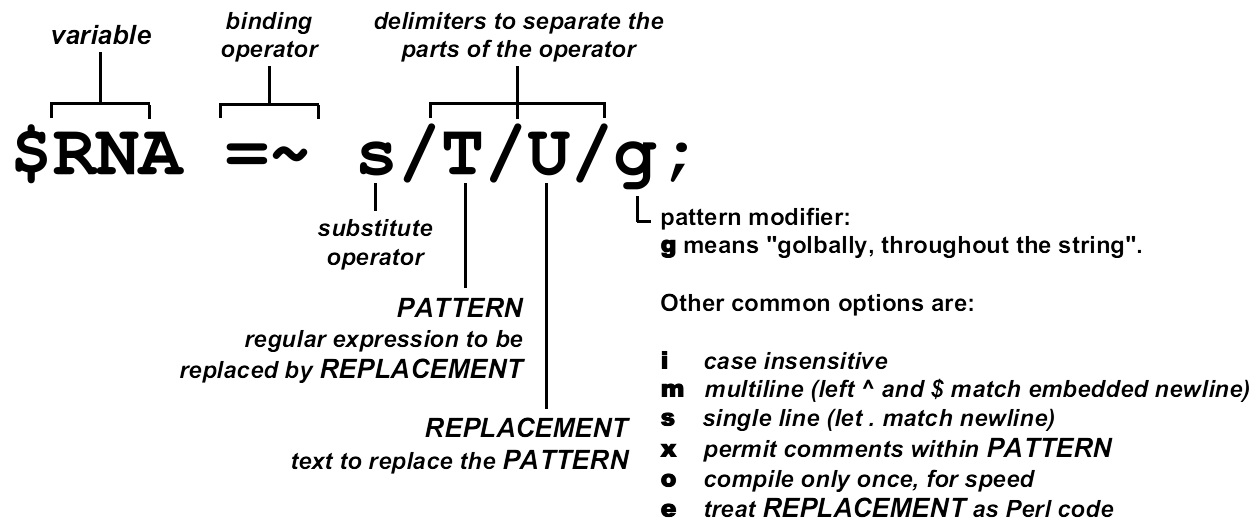
\includegraphics[width=15cm]{figure4.1.png}
  \caption{The substitution operator}
  \label{fig:figure4.1}
\end{figure}

Thus, the meaning of the statement is: "substitute all \verb|T|'s for \verb|U|'s in the string data stored in the variable \verb|$RNA|."

The substitution operator is an example of the use of regular expressions. Regular expressions are the key to text manipulation, one of the most powerful features of Perl as you'll see in later chapters. 

\section{Using the Perl Documentation}
A Perl programmer's most important resource is the Perl documentation.  It should be installed on your computer, and it may also be found on the Internet at the Perl site. The Perl documentation may come in slightly different forms on your computer system, but the web version is the same for everybody. That's the version I refer to in this book. See the references in \autoref{chap:chapteraa} for more discussion about different sources of Perl documentation.

Just to try it out, let's look up the print operator. First, open your web browser, and go to \href{http://www.perl.com}{http://www.perl.com}. Then click on the Documentation link. Select "Perl's Builtin Functions" and then "Alphabetical Listing of Perl's Functions". You'll see a rather lengthy alphabetical listing of Perl's functions. Once you've found this page, you may want to bookmark it in your browser, as you may find yourself turning to it frequently. Now click on Print to view the \verb|print| operator.

Check out the examples they give to see how the language feature is actually used. This is usually the quickest way to extract what you need to know.

Once you've got the documentation on your screen, you may find that reading it answers some questions but raises others. The documentation tends to give the entire story in a concise form, and this can be daunting for beginners. For instance, the documentation for the \verb|print| function starts out: "Prints a string or a comma-separated list of strings. Returns TRUE if successful." But then comes a bunch of gibberish (or so it seems at this point in your learning curve!) Filehandles? Output streams? List context?

All this information is necessary in documentation; after all, you need to get the whole story somewhere! Usually you can ignore what doesn't make sense.

The Perl documentation also includes several tutorials that can be a great help in learning Perl. They occasionally assume more than a beginner's knowledge about programming languages, but you may find them very useful. Exploring the documentation is a great way to get up to speed on the Perl language. 

\section{Calculating the Reverse Complement in Perl}
As you recall from \autoref{chap:chapter1}, a DNA polymer is composed of nucleotides.  Given the close relationship between the two strands of DNA in a double helix, it turns out that it's pretty straightforward to write a program that, given one strand, prints out the other. Such a calculation is an important part of many bioinformatics applications. For instance, when searching a database with some query DNA, it is common to automatically search for the reverse complement of the query as well, since you may have in hand the opposite strand of some known gene.

Without further ado, here's \autoref{exam:example4.4}, which uses a few new Perl features. As you'll see, it first tries one method, which fails, and then tries another method, which succeeds. 

\textbf{Example 4-4. Calculating the reverse complement of a strand of DNA}

\lstinputlisting[label=exam:example4.4]{./scripts/example4-4.pl}

Here's what the output of Example 4-4 should look like on your screen:

\begin{lstlisting}
Here is the starting DNA:

ACGGGAGGACGGGAAAATTACTACGGCATTAGC

Here is the reverse complement DNA:

GGAAAAGGGGAAGAAAAAAAGGGGAGGAGGGGA

That was a bad algorithm, and the reverse complement was wrong!
Try again ...

Here is the reverse complement DNA:

GCTAATGCCGTAGTAATTTTCCCGTCCTCCCGT

This time it worked!
\end{lstlisting}

You can check if two strands of DNA are reverse complements of each other by reading one left to right, and the other right to left, that is, by starting at different ends. Then compare each pair of bases as you read the two strands: they should always be paired C to G and A to T.

Just by reading in a few characters from the starting DNA and the reverse complement DNA from the first attempt, you'll see the that first attempt at calculating the reverse complement failed. It was a bad algorithm.

This is a taste of what you'll sometimes experience as you program. You'll write a program to accomplish a job and then find it didn't work as you expected. In this case, we used parts of the language we already knew and tried to stretch them to handle a new problem. Only they weren't quite up to the job. What went wrong?

You'll find that this kind of experience becomes familiar: you write some code, and it doesn't work! So you either fix the syntax (that's usually the easy part and can be done from the clues the error messages provide), or you think about the problem some more, find why the program failed, and then try to devise a new and successful way. Often this requires browsing the language documentation, looking for the details of how the language works and hoping to find a feature that fixes the problem. If it can be solved on a computer, you can solve it using Perl. The trick is, how exactly? 

In \autoref{exam:example4.4}, the first attempt to calculate the reverse complement failed. Each base in the string was translated as a whole, using four substitutions in a global fashion. Another way is needed. You could march though the DNA left to right, look at each base one at a time, make the change to the complement, and then look at the next base in the DNA, marching on to the end of the string. Then just reverse the string, and you're done. In fact, this is a perfectly good method, and it's not hard to do in Perl, although it requires some parts of the language not found until \autoref{chap:chapter5}.

However, in this case, the tr operator—which stands for transliterate or translation—is exactly suited for this task. It looks like the substitute command, with the three forward slashes separating the different parts.

\textit{tr} does exactly what's needed; it translates a set of characters into new characters, all at once. \autoref{fig:figure4.2} shows how it works: the set of characters to be translated are between the first two forward slashes. The set of characters that replaces the originals are between the second and third forward slashes. Each character in the first set is translated into the character at the same position in the second set. For instance, in \autoref{exam:example4.4}, \verb|C| is the second character in the first set, so it's translated into the second character of the second set, namely, \verb|G|.  Finally, since DNA sequence data can use upper- or lowercase letters (even though in this program the DNA is in uppercase only), both cases are included in the \textit{tr} statement in \autoref{exam:example4.4}.

\begin{figure}
  \centering
  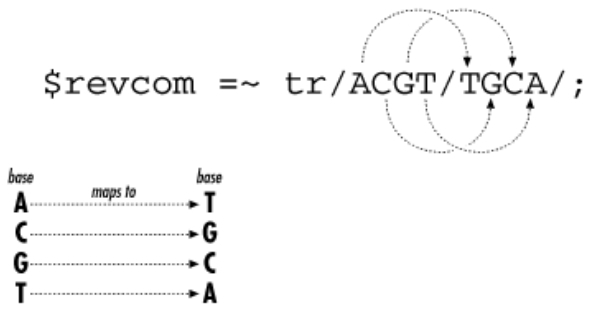
\includegraphics[width=10cm]{figure4.2.png}
  \caption{The tr statement}
  \label{fig:figure4.2}
\end{figure}

The \verb|reverse| function also does exactly what's needed, with a minimum of fuss. It's designed to reverse the order of elements, including strings as seen in \autoref{exam:example4.4}.

\section{Proteins, Files, and Arrays}
So far we've been writing programs with DNA sequence data. Now we'll also include the equally important protein sequence data. Here's an overview of what is covered in the following sections:

\begin{itemize}
  \item How to use protein sequence data in a Perl program
  \item How to read protein sequence data in from a file
  \item Arrays in the Perl language
\end{itemize}

For the rest of the chapter, both protein and DNA sequence data are used. 

\section{Reading Proteins in Files}
Programs interact with files on a computer disk. These files can be on hard disk, CD, floppy disk, Zip drive, magnetic tape—any kind of permanent storage.

Let's take a look at how to read protein sequence data from a file.  First, create a file on your computer (use your text editor) and put some protein sequence data into it. Call the file \textit{NM\_021964fragment.pep} (you can download it from this book's web site).  You will be using the following data (part of the human zinc finger protein NM\_021964):

\begin{verbatim}
MNIDDKLEGLFLKCGGIDEMQSSRTMVVMGGVSGQSTVSGELQD
SVLQDRSMPHQEILAADEVLQESEMRQQDMISHDELMVHEETVKNDEEQMETHERLPQ
GLQYALNVPISVKQEITFTDVSEQLMRDKKQIR
\end{verbatim}

You can use any name, except one that's already in use in the same folder.

Just as well-chosen variable names can be critical to understanding a program, well-chosen file and folder names can also be critical. If you have a project that generates lots of computer files, you need to carefully consider how to name and organize the files and folders. This is as true for individual researchers as for large, multi-national teams. It's important to put some effort into assigning informative names to files.

The filename \textit{NM\_021964fragment.pep} is taken from the GenBank ID of the record where this protein is found. It also indicates the fragmentary nature of the data and contains the filename extension .pep to remind you that the file contains peptide or protein sequence data. Of course, some other scheme might work better for you; the point is to get some idea of what's in the file without having to look into it.

Now that you've created or downloaded a file with protein sequence data in it, let's develop a program that reads the protein sequence data from the file and stores it into a variable. \autoref{exam:example4.5} shows a first attempt, which will be added to as we progress.

\textbf{Example 4-5. Reading protein sequence data from a file}

\lstinputlisting[label=exam:example4.5]{./scripts/example4-5.pl}

Here's the output of \autoref{exam:example4.5}:

\begin{lstlisting}
Here is the protein:

MNIDDKLEGLFLKCGGIDEMQSSRTMVVMGGVSGQSTVSGELQD
\end{lstlisting}

Notice that only the first line of the file prints out. I'll show why in a moment.

Let's look at \autoref{exam:example4.5} in more detail. After putting a filename into the variable \verb|$proteinfilename|, the file is opened with the following statement:

\begin{lstlisting}
open(PROTEINFILE, $proteinfilename);
\end{lstlisting}

After opening the file, you can do various things with it, such as reading, writing, searching, going to a specific location in the file, erasing everything in the file, and so on. Notice that the program assumes the file named in the variable \verb|$proteinfilename| exists and can be opened. You'll see in a little bit how to check for that, but here's something to try: change the name of the filename in \verb|$proteinfilename| so that there's no file of that name on your computer, and then run the program. You'll get some error messages if the file doesn't exist.

If you look at the documentation for the \verb|open| function, you'll see many options. Mostly, they enable you to specify exactly what the file will be used for after it's opened.

Let's examine the term \verb|PROTEINFILE|, which is called a \textit{filehandle}. With filehandles, it's not important to understand what they really are.  They're just things you use when you're dealing with files. They don't have to have capital letters, but it's a widely followed convention.  After the open statement assigns a filehandle, all the interaction with a file is done by naming the filehandle.  

The data is actually read in to the program with the statement:

\begin{lstlisting}
$protein = <PROTEINFILE>;
\end{lstlisting}

Why is the filehandle \verb|PROTEINFILE| enclosed within angle brackets? These angle brackets are called \textit{input operators}; a filehandle within angle brackets is how you bring in data from some source outside the program.  Here, we're reading the file called \verb|NM\_021964fragment.pep| whose name is stored in variable \verb|$proteinfilename|, and which has a filehandle associated with it by the open statement. The data is being stored in the variable \verb|$protein| and then printed out.

However, as you've already noticed, only the first line of this multiline file is printed out. Why? Because there are a few more things to learn about reading in files.

There are several ways to read in a whole file. \autoref{exam:example4.6} shows one way.

\textbf{Example 4-6. Reading protein sequence data from a file, take 2}

\lstinputlisting[label=exam:example4.6]{./scripts/example4-6.pl}

Here's the output of Example 4-6:

\begin{lstlisting}
Here is the first line of the protein file:

MNIDDKLEGLFLKCGGIDEMQSSRTMVVMGGVSGQSTVSGELQD

Here is the second line of the protein file:

SVLQDRSMPHQEILAADEVLQESEMRQQDMISHDELMVHEETVKNDEEQMETHERLPQ

Here is the third line of the protein file:

GLQYALNVPISVKQEITFTDVSEQLMRDKKQIR
\end{lstlisting}

The interesting thing about this program is that it shows how reading from a file works. Every time you read into a scalar variable such as \verb|$protein|, the next line of the file is read. Something is remembering where the previous read was and is picking it up from there.

On the other hand, the drawbacks of this program are obvious. Having to write a few lines of code for each line of an input file isn't convenient. However, there are two Perl features that can handle this nicely: arrays (in the next section) and loops (in \autoref{chap:chapter5}). 

\section{Arrays}
In computer languages an array is a variable that stores multiple scalar values. The values can be numbers, strings, or, in this case, lines of an input file of protein sequence data. Let's examine how they can be used. \autoref{exam:example4.7} shows how to use an array to read all the lines of an input file.

\textbf{Example 4-7. Reading protein sequence data from a file, take 3}

\lstinputlisting[label=exam:example4.7]{./scripts/example4-7.pl}

Here's the output of Example 4-7:

\begin{lstlisting}
MNIDDKLEGLFLKCGGIDEMQSSRTMVVMGGVSGQSTVSGELQD
SVLQDRSMPHQEILAADEVLQESEMRQQDMISHDELMVHEETVKNDEEQMETHERLPQ
GLQYALNVPISVKQEITFTDVSEQLMRDKKQIR
\end{lstlisting}

which, as you can see, is exactly the data that's in the file. Success!

The convenience of this is clear—just one line to read all the data into the program. 

Notice that the array variable starts with an at sign (@) rather than the dollar sign (\$) scalar variables begin with. Also notice that the \verb|print| function can handle arrays as well as scalar variables. Arrays are used a lot in Perl, so you will see plenty of array examples as the book continues.  

An array is a variable that can hold many scalar values. Each item or element is a scalar value that can be referenced by giving its position in the array (its subscript or offset). Let's look at some examples of arrays and their most common operations. We'll define an array \verb|@bases| that holds the four bases A, C, G, and T. Then we'll apply some of the most common array operators.

Here's a piece of code that demonstrates how to initialize an array and how to use subscripts to access the individual elements of an array: 

\begin{lstlisting}
# Here's one way to declare an array, initialized with a list of four scalar values.
@bases = ('A', 'C', 'G', 'T');

# Now we'll print each element of the array
print "Here are the array elements:";
print "\nFirst element: ";
print $bases[0];
print "\nSecond element: ";
print $bases[1];
print "\nThird element: ";
print $bases[2];
print "\nFourth element: ";
print $bases[3];
\end{lstlisting}

This code snippet prints out:

\begin{lstlisting}
First element: A
Second element: C
Third element: G
Fourth element: T
\end{lstlisting}

You can print the elements one a after another like this:

\begin{lstlisting}
@bases = ('A', 'C', 'G', 'T');
print "\n\nHere are the array elements: ";
print @bases;
\end{lstlisting}

which produces the output:

\begin{lstlisting}
Here are the array elements: ACGT
\end{lstlisting}

You can also print the elements separated by spaces (notice the double quotes in the \verb|print| statement): 

\begin{lstlisting}
@bases = ('A', 'C', 'G', 'T');
print "\n\nHere are the array elements: ";
print "@bases";
\end{lstlisting}

which produces the output:

\begin{lstlisting}
Here are the array elements: A C G T
\end{lstlisting}

You can take an element off the end of an array with \verb|pop|: 

\begin{lstlisting}
@bases = ('A', 'C', 'G', 'T');
$base1 = pop @bases;
print "Here's the element removed from the end: ";
print $base1, "\n\n";
print "Here's the remaining array of bases: ";
print "@bases";
\end{lstlisting}

which produces the output:

\begin{lstlisting}
Here's the element removed from the end: T

Here's the remaining array of bases: A C G
\end{lstlisting}

You can take a base off of the beginning of the array with \verb|shift|:

\begin{lstlisting}
@bases = ('A', 'C', 'G', 'T');
$base2 = shift @bases;
print "Here's an element removed from the beginning: ";
print $base2, "\n\n";
print "Here's the remaining array of bases: ";
print "@bases";
\end{lstlisting}

which produces the output:

\begin{lstlisting}
Here's an element removed from the beginning: A

Here's the remaining array of bases: C G T
\end{lstlisting}

You can put an element at the beginning of the array with \verb|unshift|: 

\begin{lstlisting}
@bases = ('A', 'C', 'G', 'T');
$base1 = pop @bases;
unshift (@bases, $base1);
print "Here's the element from the end put on the beginning: ";
print "@bases\n\n";
\end{lstlisting}

which produces the output:

\begin{lstlisting}
Here's the element from the end put on the beginning: T A C G
\end{lstlisting}

You can put an element on the end of the array with \verb|push|: 

\begin{lstlisting}
@bases = ('A', 'C', 'G', 'T');
$base2 = shift @bases;
push (@bases, $base2);
print "Here's the element from the beginning put on the end: ";
print "@bases\n\n";
\end{lstlisting}

which produces the output:

\begin{lstlisting}
Here's the element from the beginning put on the end: C G T A
\end{lstlisting}

You can reverse the array: 

\begin{lstlisting}
@bases = ('A', 'C', 'G', 'T');
@reverse = reverse @bases;
print "Here's the array in reverse: ";
print "@reverse\n\n";
\end{lstlisting}

which produces the output:

\begin{lstlisting}
Here's the array in reverse: T G C A
\end{lstlisting}

You can get the length of an array:

\begin{lstlisting}
@bases = ('A', 'C', 'G', 'T');
print "Here's the length of the array: ";
print scalar @bases, "\n";
\end{lstlisting}

which produces the output:

\begin{lstlisting}
Here's the length of the array: 4
\end{lstlisting}

Here's how to insert an element at an arbitrary place in an array using the Perl \verb|splice| function: 

\begin{lstlisting}
@bases = ('A', 'C', 'G', 'T');
splice ( @bases, 2, 0, 'X' );
print "Here's the array with an element inserted after the 2nd element: ";
print "@bases\n";
\end{lstlisting}

which produces the output:

\begin{lstlisting}
Here's the array with an element inserted after the 2nd element: A C X G T
\end{lstlisting}

\section{Scalar and List Context}
Many Perl operations behave differently depending on the context in which they are used. Perl has \textit{scalar context} and \textit{list context}; both are listed in \autoref{exam:example4.8}.

\textbf{Example 4-8. Scalar context and list context}

\lstinputlisting[label=exam:example4.8]{./scripts/example4-8.pl}

Here's the output of \autoref{exam:example4.8}:

\begin{lstlisting}
A C G T
4
A
\end{lstlisting}

First, \autoref{exam:example4.8} declares an array of the four bases. Then the assignment statement tries to assign an array (which is a kind of list) to a scalar variable \verb|$a|: 

\begin{lstlisting}
$a = @bases;
\end{lstlisting}

In this kind of \textit{scalar context}, an array evaluates to the size of the array, that is, the number of elements in the array. The scalar context is supplied by the scalar variable on the left side of the statement.

Next, \autoref{exam:example4.8} tries to assign an array (to repeat, a kind of list) to another list, in this case, having just one variable, \verb|$a|:

\begin{lstlisting}
($a) = @bases;
\end{lstlisting}

In this kind of \textit{list context}, an array evaluates to a list of its elements. The list context is supplied by the list in parentheses on the left side of the statement. If there aren't enough variables on the left side to assign to, only part of the array gets assigned to variables.  This behavior of Perl pops up in many situations; by design, many features of Perl behave differently depending on whether they are in scalar or list context. See \autoref{chap:chapterab} for more about scalar and list content.

Now you've seen the use of strings and arrays to hold sequence and file data, and learned the basic syntax of Perl, including variables, assignment, printing, and reading files. You've transcribed DNA to RNA and calculated the reverse complement of a strand of DNA. By the end of \autoref{chap:chapter5}, you'll have covered the essentials of Perl programming. 

\section{Exercises}
\textcolor{red}{\textit{Exercise 4.1}}
\begin{adjustwidth}{1cm}{}
Explore the sensitivity of programming languages to errors of syntax.  Try removing the semicolon from the end of any statement of one of our working programs and examining the error messages that result, if any.  Try changing other syntactical items: add a parenthesis or a curly brace; misspell "print" or some other reserved word; just type in, or delete, anything. Programmers get used to seeing such errors; even after getting to know the language well, it is still common to have some syntax errors as you gradually add code to a program. Notice how one error can lead to many lines of error reporting. Is Perl accurately reporting the line where the error is? 
\end{adjustwidth}

\textcolor{red}{\textit{Exercise 4.2}}
\begin{adjustwidth}{1cm}{}
Write a program that stores an integer in a variable and then prints it out. 
\end{adjustwidth}

\textcolor{red}{\textit{Exercise 4.3}}
\begin{adjustwidth}{1cm}{}
Write a program that prints DNA (which could be in upper- or lowercase originally) in lowercase (acgt); write another that prints the DNA in uppercase (ACGT). Use the function \textit{tr///}. 
\end{adjustwidth}

\textcolor{red}{\textit{Exercise 4.4}}
\begin{adjustwidth}{1cm}{}
Do the same thing as Exercise 4.3, but use the string directives \verb|\U| and \verb|\L| for upper- and lowercase. For instance, \verb|print "\U$DNA"| prints the data in \verb|$DNA| in uppercase. 
\end{adjustwidth}

\textcolor{red}{\textit{Exercise 4.5}}
\begin{adjustwidth}{1cm}{}
Sometimes information flows from RNA to DNA. Write a program to reverse transcribe RNA to DNA. 
\end{adjustwidth}

\textcolor{red}{\textit{Exercise 4.6}}
\begin{adjustwidth}{1cm}{}
Read two files of data, and print the contents of the first followed by the contents of the second. 
\end{adjustwidth}

\textcolor{red}{\textit{Exercise 4.7}}
\begin{adjustwidth}{1cm}{}
This is a more difficult exercise. Write a program to read a file, and then print its lines in reverse order, the last line first. Or you may want to look up the functions \textit{push}, \textit{pop}, \textit{shift}, and \textit{unshift}, and choose one or more of them to accomplish this exercise. You may want to look ahead to \autoref{chap:chapter5} so you can use a loop in this program, but this may not be necessary depending on the approach you take. Or, you may want to use reverse on an array of lines. 
\end{adjustwidth}

